% !TEX TS-program = lualatex
% !TEX encoding = UTF-8

% This is a simple template for a LuaLaTeX document using gregorio scores.

\documentclass[letterpaper,12pt]{book} % use larger type; default would be 10pt

\input{header.inc}

\geometry{letterpaper,outer=0.4in,inner=0.9in,top=1in,bottom=0.8in}

\begin{document}
\garamondbig
\greannotation{Ant.}
\greannotation{7.}
\gregorioscore{185_an--sub_tuum_praesidium--solesmes}

\bigskip

\greannotation{1.}
\gregorioscore{185_va--ave_maria--solesmes}

\begin{centering}

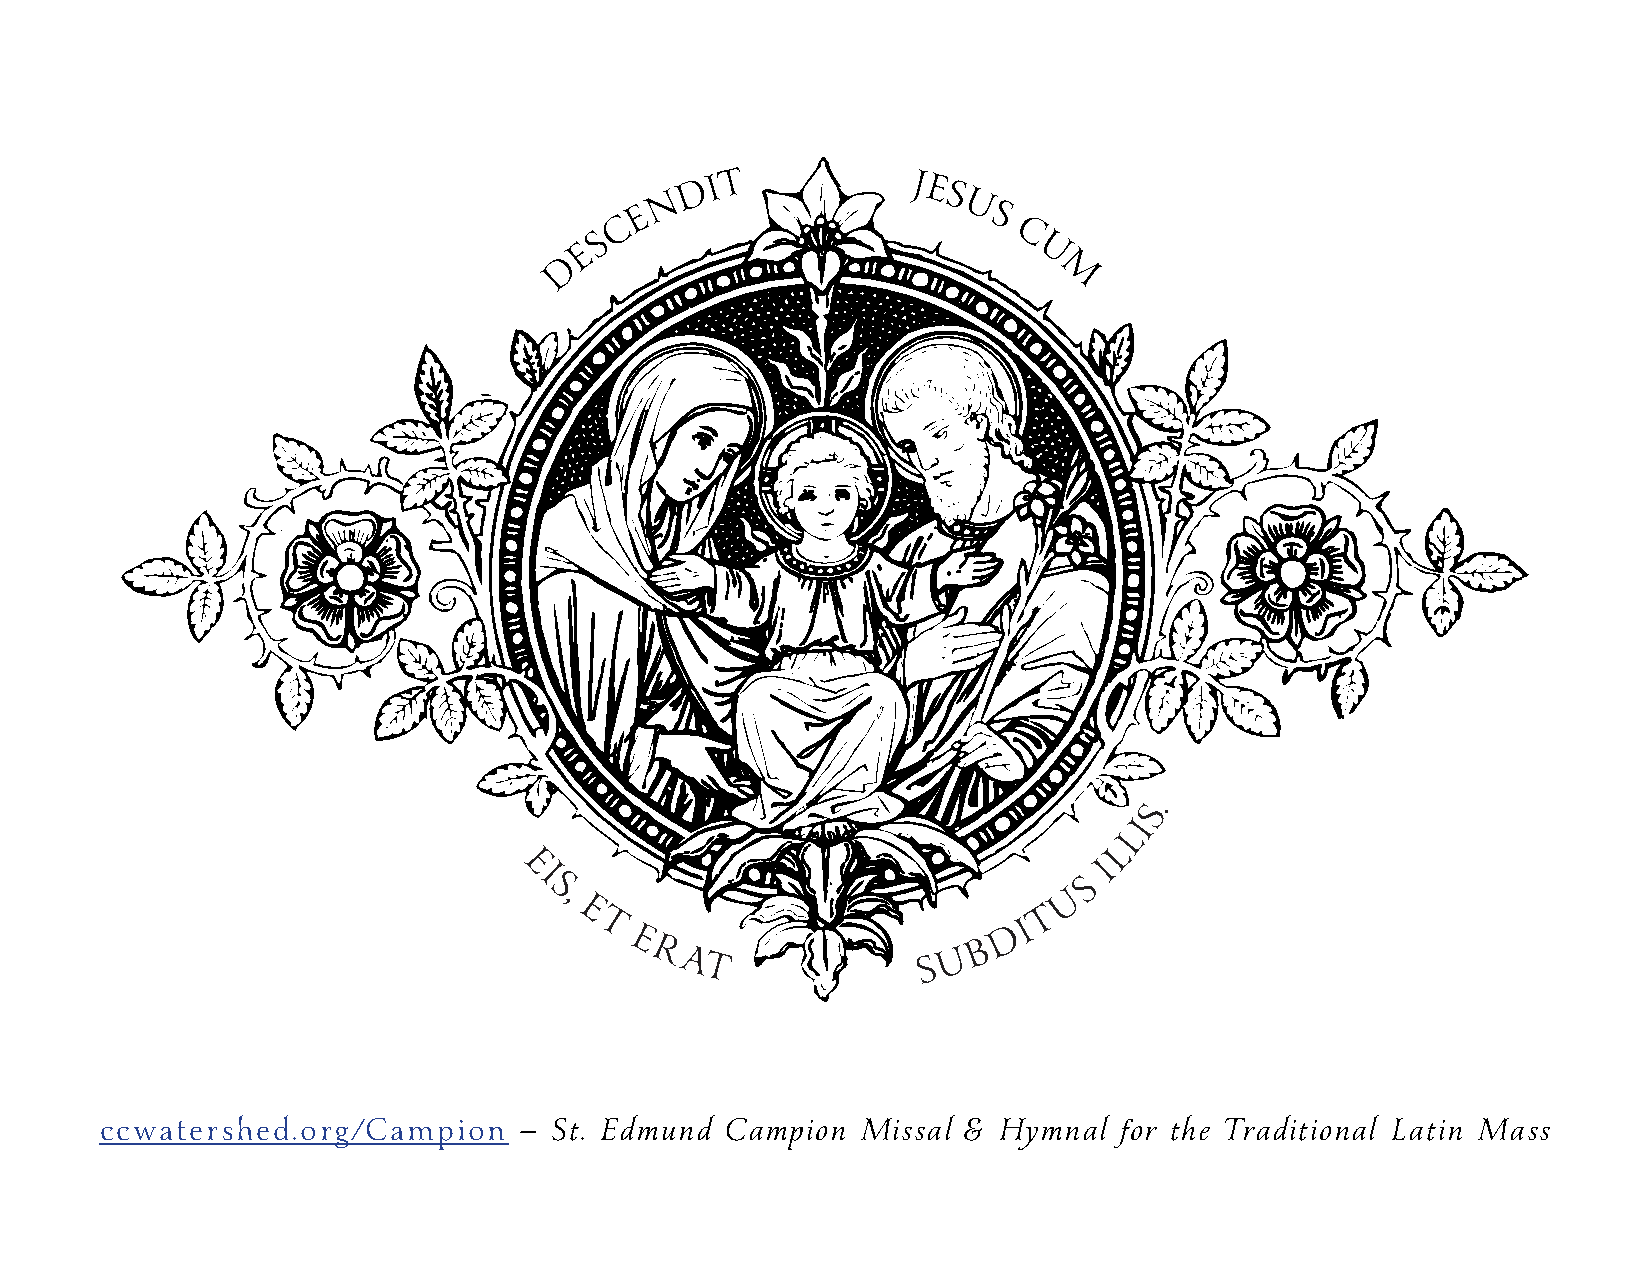
\includegraphics[clip,trim=0.8in 1.81in 0.8in 1.034in,width=0.6\textwidth]{../186_clipart.pdf}

\vfill

\end{centering}

\greannotation{Hymn.}
\greannotation{2.}
\gregorioscore{186_hy--maria_mater_gratiae--solesmes}

\end{document}